\documentclass[12pt]{article}

\usepackage[margin=1in]{geometry}
\usepackage{setspace}
\usepackage{graphicx}
\usepackage{enumitem}
\usepackage{titlesec}
\usepackage{fancyhdr}
\usepackage{xcolor}
\usepackage{tikz}
\usepackage{hyperref}
\usepackage{url}
\usepackage{natbib} 

\usetikzlibrary{shapes.geometric, arrows}
\tikzstyle{startstop} = [rectangle, rounded corners, minimum width=4cm, minimum height=1.2cm, 
                         text centered, draw=black, fill=red!30, line width=1pt]
\tikzstyle{process} = [rectangle, minimum width=4cm, minimum height=1.2cm, text centered, 
                       draw=black, fill=blue!30, line width=1pt]
\tikzstyle{io} = [trapezium, trapezium left angle=70, trapezium right angle=110, 
                  minimum width=4cm, minimum height=1.2cm, text centered, draw=black, fill=green!30, align=center, line width=1pt]
\tikzstyle{arrow} = [thick,->,>=stealth]

\hypersetup{
    colorlinks=true,
    linkcolor=black,
    citecolor=black,
    urlcolor=blue
}


\setstretch{1.25}

\hypersetup{
    colorlinks=true,
    linkcolor=black,
    urlcolor=blue
}

\setlength{\parindent}{0pt}
\setlength{\parskip}{0.6em}

\titlespacing*{\section}{0pt}{1.5em}{1em}
\titlespacing*{\subsection}{0pt}{1.2em}{0.8em}

\raggedright

\pagestyle{fancy}
\fancyhf{}
\fancyfoot[C]{\thepage}
\renewcommand{\headrulewidth}{0pt}

\titleformat{\section}
  {\Large\bfseries}
  {}
  {0pt}
  {}
  [\vspace{-0.3em}\rule{\linewidth}{0.6pt}\vspace{0.8em}]

\titleformat{\subsection}
  {\large\bfseries}d
  {}
  {0pt}
  {}

\begin{document}

\begin{titlepage}
    \centering
    \vspace*{1.8in}

    {\Huge \textbf{CardioIQ}}\\[0.3cm]
    {\Large AI-Powered Cardiovascular Risk Analysis}\\[0.8cm]

    {\large Track II -- Technical / Implementation}\\[1.5cm]

    \rule{0.85\linewidth}{0.8pt}\\[1cm]

    \textbf{Team Member}\\[0.3cm]
    Zain Aboobacker\\[0.8cm]

    \textbf{Supervising Adult}\\[0.3cm]
    Vadakummuri Aboobacker\\[0.8cm]

    \textbf{Community}\\[0.3cm]
    Natick, Massachusetts\\[1.2cm]

    Submission Date: January 19th, 2026

    \vfill
\end{titlepage}

\section*{Executive Overview}
\addcontentsline{toc}{section}{Executive Overview}
CardioIQ is an \textbf{end-to-end fully functional AI-based system designated for accurate cardiovascular risk assessment} outside a doctor’s office. The platform aims to help individuals recognize potential cardiovascular risks earlier and take meaningful action before symptoms take effect.

CardioIQ aligns with \textbf{Executive Order 14277, "Advancing Artificial Intelligence (AI) Education for American Youth"}, by translating AI education from abstract concepts into a deployed, community-facing system\cite{eo14277}. Rather than limiting AI-learning to theory, CardioIQ demonstrates how students can responsibly apply AI technology to solve real public health challenges. 

\section*{Community Problem}
\addcontentsline{toc}{section}{Community Problem}

CardioIQ was designed to address gaps in preventive cardiovascular screening in Natick, Massachusetts. In Natick, about \textbf{37.2\% of adults have hypertension}, a major risk factor for cardiovascular disease \cite{natickCHNA2025}, suggesting persistent unmet needs in screening and risk detection.


Additionally, CardioIQ was also designed to be usable in a broader, national context. Considering that cardiovascular disease accounts for the \textbf{greatest rate of deaths within the USA} and that on average, someone in the U.S. \textbf{dies from cardiovascular disease every 34 seconds }\cite{ahaCVDdeaths2025}, CardioIQ is also made to help those all around the country. 

Moreover, signs for cardiovascular disease can often be missed, especially outside clinical settings. Nationwide, about \textbf{15\% of U.S. adults report never having received any cardiovascular screening} \cite{cdcHeartScreening2024}. Many communities also lack reliable access to cardiovascular screening due to financial strain or limited healthcare resources. As a result, individuals often address their cardiovascular health only after symptoms emerge, at which point treatment may be less effective.

Without interpretable risk information, individuals are less likely to address their health or seek medical guidance. Delayed awareness can contribute to the progression of cardiovascular conditions, increasing long-term health risks for individuals.

\section*{Solution Overview}
\addcontentsline{toc}{section}{Solution Overview}

CardioIQ provides an \textbf{accessible, AI-powered solution to prevent cardiovascular disease} through interpretable risk assessment. The platform utilizes a combination of ECG data, user-input health metrics, and advanced AI algorithms in order to produce a clinically relevant cardiovascular risk. 

Unlike many consumer health applications that rely on self-reported data or static questionaires, CardioIQ directly analyzes raw ECG data in combination with lifestyle and physiological inputs. CardioIQ moves beyond basic health tracking into proactive, AI-assisted cardiovascular risk awareness. 

The core functionality includes:  

\begin{itemize}[leftmargin=1.5em]
    \item \textbf{ECG Analysis:} Automated interpretation of electrocardiogram signals to \textbf{identify potential abnormalities or irregular heart rhythms}.
    \item \textbf{Risk Modeling:} Integration of established cardiovascular risk factors (e.g., ECG abnormality, age, blood pressure, lifestyle habits) into predictive AI models that can \textbf{estimate cardiovascular risk}.
    \item \textbf{Personalized Feedback:} Generation of \textbf{clear, actionable recommendations, lifestyle guidance, and prompts for professional consultation} based on AI-driven risk assessments through the use of an AI LLM (large language model).
    \item \textbf{User-Friendly Interface:} Intuitive dashboard that visualizes predictions, risk scores, trend analysis, and ECG results.
    \item \textbf{Data Security and Privacy:} Secure handling of personal health information in compliance with relevant privacy standards, ensuring user trust and data integrity.
\end{itemize}


By combining these capabilities, CardioIQ empowers individuals in Natick and similar communities to identify potential cardiovascular risks, take action, and make informed decisions about seeking professional care. \textbf{For example, consider a 45-year-old resident of Natick} with no prior history of heart disease. After uploading an at-home ECG recording and entering basic health information into CardioIQ, the system identifies subtle ECG irregularities combined with elevated blood pressure and lifestyle risk factors. CardioIQ informs this user of their risk factors and prompts them to seek professional evaluation. Acting on this information, the individual schedules a preventive cardiology appointment, where risk factors are identified. In this way, \textbf{CardioIQ functions as an early-warning system}, enabling intervention before cardiovascular conditions become severe.

\section*{CardioIQ Workflow Diagram}
\addcontentsline{toc}{section}{CardioIQ Workflow Diagram}

\begin{center}
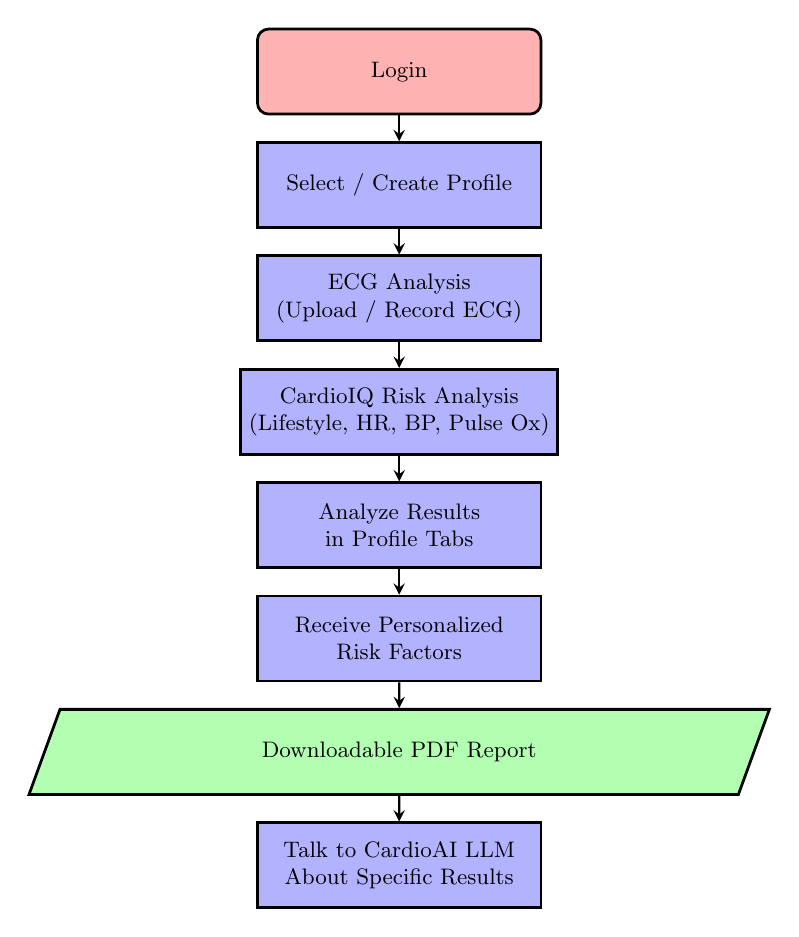
\begin{tikzpicture}[node distance=1.6cm, every node/.style={font=\small}, scale=0.9, transform shape]

\node (login) [startstop] {Login};
\node (profile) [process, below of=login] {Select / Create Profile};
\node (ecg) [process, below of=profile, align=center] {ECG Analysis \\ (Upload / Record ECG)};
\node (risk) [process, below of=ecg, align=center] {CardioIQ Risk Analysis \\ (Lifestyle, HR, BP, Pulse Ox)};
\node (results) [process, below of=risk, align=center] {Analyze Results \\ in Profile Tabs};
\node (riskfactors) [process, below of=results, align=center] {Receive Personalized \\ Risk Factors};
\node (pdf) [io, below of=riskfactors, align=center] {Downloadable PDF Report};
\node (chat) [process, below of=pdf, align=center] {Talk to CardioAI LLM \\ About Specific Results};

\draw [arrow] (login) -- (profile);
\draw [arrow] (profile) -- (ecg);
\draw [arrow] (ecg) -- (risk);
\draw [arrow] (risk) -- (results);
\draw [arrow] (results) -- (riskfactors);
\draw [arrow] (riskfactors) -- (pdf);
\draw [arrow] (pdf) -- (chat);

\end{tikzpicture}
\end{center}
\section*{AI Methods and Technologies}
\addcontentsline{toc}{section}{AI Methods and Technologies}

CardioIQ uses multiple AI technologies to provide comprehensive cardiovascular analysis. 

\begin{itemize}[leftmargin=1.5em]
    \item \textbf{ECGNet - Residual Convolutional Neural Network (CNN):} Optimized for ECGs, the model is used to analyze ECG signals, this AI model can detect patterns and irregularities in heart activity that may indicate risk using ECGs, even when subtle or difficult for non-experts to see.
    \item \textbf{CardioRiskNet - Multilayer Perceptron (MLP):} A machine learning model that evaluates key cardiovascular risk factors, such as blood pressure, heart rate, age, lifestyle, and ECG results to generate an accurate personalized risk score.
    \item \textbf{CardioAI - Liquid LFM-1.2B - AI Language Model (LLM):} A computationally efficient LLM that provides clear, understandable feedback and recommendations to users, translating complex results into guidance while prompting the user to seek medical attention when necessary.
\end{itemize}

By combining these AI methods, CardioIQ transforms raw data and health information into actionable insights, allowing users to make informed decisions about their cardiovascular health without needing medical knowledge.

\section*{Development Process and Challenges}
\addcontentsline{toc}{section}{Development Process and Challenges}

During the development of CardioIQ, several challenges required solutions to ensure accuracy, usability, and performance:  

An early challenge involved \textbf{noisy ECG signals}, which significantly \textbf{reduced initial model performance}. Early training runs produced incorrect classifications due to noisy artifacts that the model was not tuned to handle. To address this, \textbf{ECG-specific data augmentation} was implemented, a technique designed to increase signal diversity and improve the models ability to generalize on real-world data. 

Additionally, integrating ECG interpretation, risk modeling, and personalized feedback into \textbf{one coherent interface} was a big challenge. At first, early prototypes fragmented these components, creating a cluttered and hard-to-follow application. This problem was solved through recurrent redesigns of the interface, allowing each AI component to fit into a unified app, \textbf{allowing users to clearly navigate the platform and understand their cardiovascular results}. 

\textbf{Computational limitations} also limited the use of large langauage models for personalized feedback. Initial experiments used large models that proved extremely slow and computationally intensive. This led to the adoption of Liquid LFM-1.2B, an LLM specifically designed for quick and efficient inference that proved effective in providing clinically relevant explanations, enabling \textbf{scalable inference without sacrificing output quality.} 

These solutions allowed CardioIQ to provide accurate and user-friendly cardiovascular insights despite the challenges in working with complex medical data and AI.

\section*{Testing, Validation, and Accuracy}
\addcontentsline{toc}{section}{Testing, Validation, and Accuracy}

CardioIQ underwent \textbf{rigorous testing} to ensure that its predictions were both accurate and reliable.  

\begin{itemize}[leftmargin=1.5em]
    \item \textbf{ECG Analysis Accuracy:} ECGNet, was trained on a diverse set of ECG signals. After 150 epochs, the model achieved a best F1 score of 0.84 at a threshold of 0.86, with precision of 0.77, recall of 0.84, PR-AUC of 0.88, and ROC-AUC of 0.99. This demonstrates that the model can accurately identify abnormal heart patterns while minimizing false alarms.
    \item \textbf{Cardiovascular Risk Modeling:} CardioRiskNet achieved a final loss of 0.0009, indicating reliable predictions based on user-input health metrics. Compared to a rule-based baseline, CardioRiskNet showed significantly improved stability and accuracy across diverse profiles.
    \item \textbf{LLM Feedback Validation:} LiquidLFM provided personalized feedback which was tested under specific restrictions to ensure that all responses are safe and medically relevant. 
    \item \textbf{Overall System Testing:} The full app was tested end-to-end with sample user data to verify that ECG analysis, risk scoring, and feedback generation functioned correctly together and produced safe, actionable results.
\end{itemize}

Through this rigorous evaluation, CardioIQ demonstrates \textbf{strong performance, safe user guidance, and reliability in real-world scenarios.}

\section*{Responsible and Ethical Use of AI}
\addcontentsline{toc}{section}{Responsible and Ethical Use of AI}

CardioIQ implements \textbf{safeguards to ensure ethical use of AI}, including safe LLM outputs, secure data storage, hard-coded medical disclaimers, refusal logic for diagnosis, and clear guidance that AI is a support tool and not a replacement for medical professionals. 


\section*{Learning Outcomes and Reflection}
\addcontentsline{toc}{section}{Learning Outcomes and Reflection}

Creating CardioIQ increased my understanding of both the \textbf{potiential and limitations of applying AI in healthcare}. While developing the ECG and risk models, I learned that strong performance metrics aren't enough to justify use in a medical setting. Careful validation and safeguards are also needed for responsible use. Additionally, small design choices, such as how risk scores are explained or when users are prompted to seek medical attention, can significantly affect how individuals respond to AI-generated insights. 

This project also taught me the importance continous improvements over time. Through this process, I gained a clear understanding of how \textbf{AI systems should be continously refined and improved}, especially in health-related contexts. 

Throughout the development of this project, I've also gained a deeper insight into my future. I've truly learned how my passion for AI can can evolve into true change. From now on, I aspire to innovate and advance by \textbf{improving healthcare and improving quality of life in this country.}
 
\section*{Future Improvements and Scalability}
\addcontentsline{toc}{section}{Future Improvements and Scalability}

In the future, the development of CardioIQ will be directed towards developing its capabilities further in order for the system to be even more accurate and beneficial.

One possible improvement is \textbf{device integration}. This would enable patients to automatically log readings related to ECGs, blood pressure, heart rate, and blood oxygen levels at home. It's important to note, however, that these devices would increase cost of the product. Nevertheless, the cost of these devices would be far less than often unnecessary doctor visits that are extremely expensive. Ultimately, this would streamline data collection and provide a complete picture of cardiovascular health without requiring manual input. 

Additionally, the AI models can be further refined for better accuracy and efficiency. Through constant, iterative improvements, CardioIQ can deliver even more reliable risk assessments while remaining user-friendly.  

Beyond feature-enhancement, CardioIQ is also a designated \textbf{web-accessible application}. Future development will also be focused on \textbf{scaling} the platform into a robust, internet-based health system capable of supporting a large-scale userbase. One key improvement is moving into cloud-based architectures. This would allow computational resources to adjust based on user demand. This would enable real-time inference for thousands of users at the same time. 

These enhancements will make the platform more accurate and reliable, allowing more individuals to monitor and manage their cardiovascular health.

\section*{Video}
\addcontentsline{toc}{section}{Video}

The submission video for CardioIQ is included here:  \href{https://www.youtube.com/watch?v=BUGhDGgTrsQ}{CardioIQ Submission Video}

\section*{Conclusion}
\addcontentsline{toc}{section}{Conclusion}

CardioIQ shows how \textbf{AI can help cardiovascular health through accurate and actionable insights}. While challenges remain, the platform shows that combining ECG analysis, risk modeling, and personalized guidance can make proactive health management simpler and more effective. With more refinement and integration of devices, CardioIQ has the potential to save lives.

\section*{Certification of Originality}
\addcontentsline{toc}{section}{Certification of Originality}

We certify that this project submission is original work created specifically for the Presidential AI Challenge. All AI tools, datasets, and external resources used have been fully identified and credited.

\vspace{0.8cm}
\noindent\textbf{Team Member Signature:}\\
Zain Aboobacker

\section*{Tool Attribution}
\addcontentsline{toc}{section}{References and Tool Attribution}

\begin{itemize}[leftmargin=1.5em]
    \item Moody GB, Mark RG. The Impact of the MIT-BIH Arrhythmia Database. \textit{IEEE Engineering in Medicine and Biology Magazine, May–Jun 2001.} Dataset used for ECG model training and evaluation. \href{https://www.physionet.org/content/mitdb/1.0.0/}{MIT-BIH Arrhythmia Database}
    \item Software Libraries: TensorFlow / PyTorch / Numpy / Pandas - Frameworks used for model development.
    \item AI Tools and Platforms: LM Studio - Used for accessing Liquid LFM-1.2B LLM for personalized feedback.
\end{itemize}

\section*{Code Availability}
\addcontentsline{toc}{section}{Code Availability}
All source code, datasets, and scripts used in this project are publicly available on GitHub: 
\href{https://github.com/yourusername/CardioIQ}{https://github.com/yourusername/CardioIQ}.

\bibliographystyle{plain} 
\bibliography{references}

\end{document}
